% TeX eps-loader file generated by stoch_simul.m (Dynare).
% 12-Feb-2024 14:16:17
 
\begin{figure}[H]
\centering 
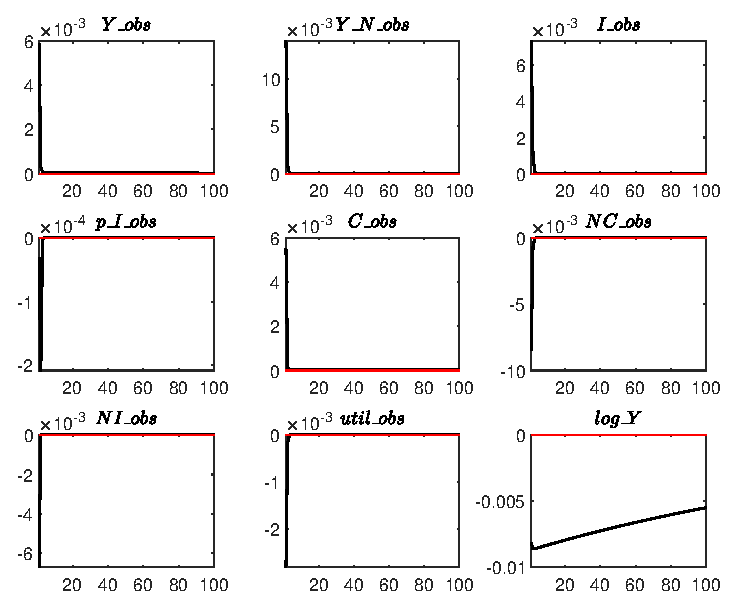
\includegraphics[width=0.80\textwidth]{BRS_imp_mobility_alt/graphs/BRS_imp_mobility_alt_IRF_e_g1}
\caption{Impulse response functions (orthogonalized shock to ${e_g}$).}\label{Fig:IRF:e_g:1}
\end{figure}
 
\begin{figure}[H]
\centering 
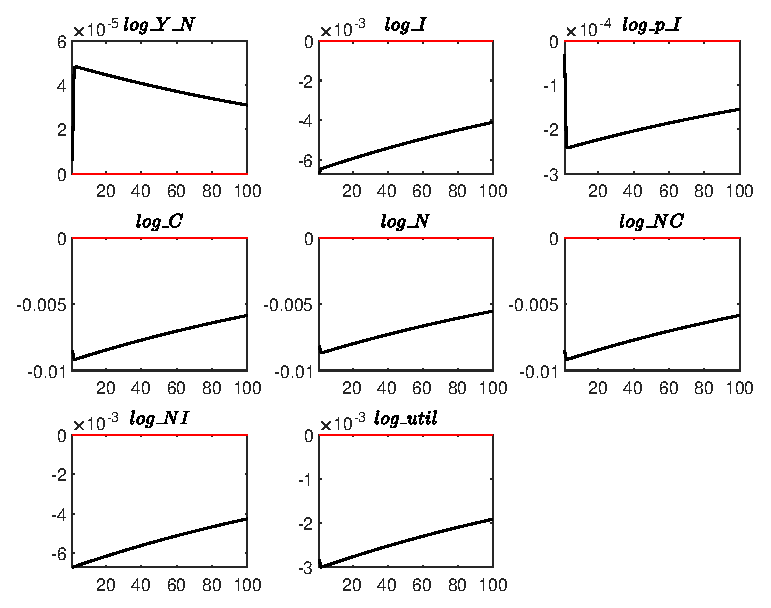
\includegraphics[width=0.80\textwidth]{BRS_imp_mobility_alt/graphs/BRS_imp_mobility_alt_IRF_e_g2}
\caption{Impulse response functions (orthogonalized shock to ${e_g}$).}\label{Fig:IRF:e_g:2}
\end{figure}
 
\begin{figure}[H]
\centering 
\includegraphics[width=0.80\textwidth]{BRS_imp_mobility_alt/graphs/BRS_imp_mobility_alt_IRF_e_ZI1}
\caption{Impulse response functions (orthogonalized shock to ${e_{ZI}}$).}\label{Fig:IRF:e_ZI:1}
\end{figure}
 
\begin{figure}[H]
\centering 
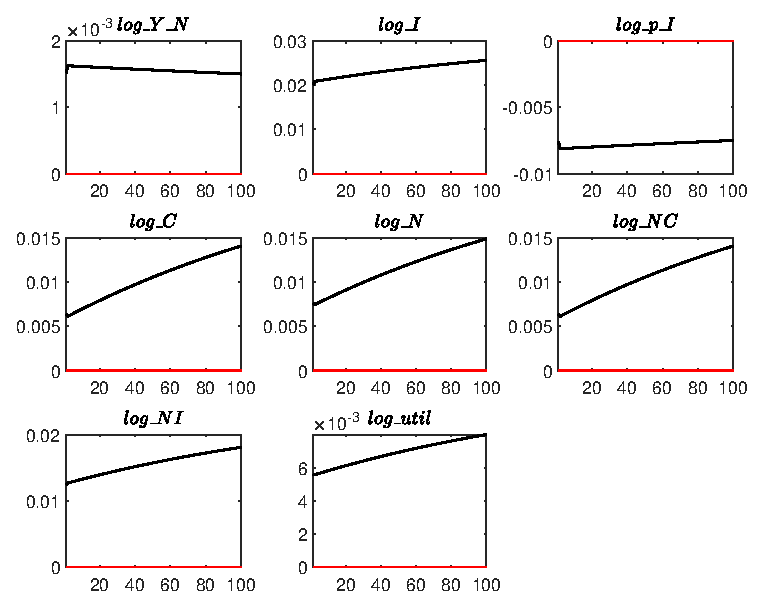
\includegraphics[width=0.80\textwidth]{BRS_imp_mobility_alt/graphs/BRS_imp_mobility_alt_IRF_e_ZI2}
\caption{Impulse response functions (orthogonalized shock to ${e_{ZI}}$).}\label{Fig:IRF:e_ZI:2}
\end{figure}
 
\begin{figure}[H]
\centering 
\includegraphics[width=0.80\textwidth]{BRS_imp_mobility_alt/graphs/BRS_imp_mobility_alt_IRF_e_N1}
\caption{Impulse response functions (orthogonalized shock to ${e_N}$).}\label{Fig:IRF:e_N:1}
\end{figure}
 
\begin{figure}[H]
\centering 
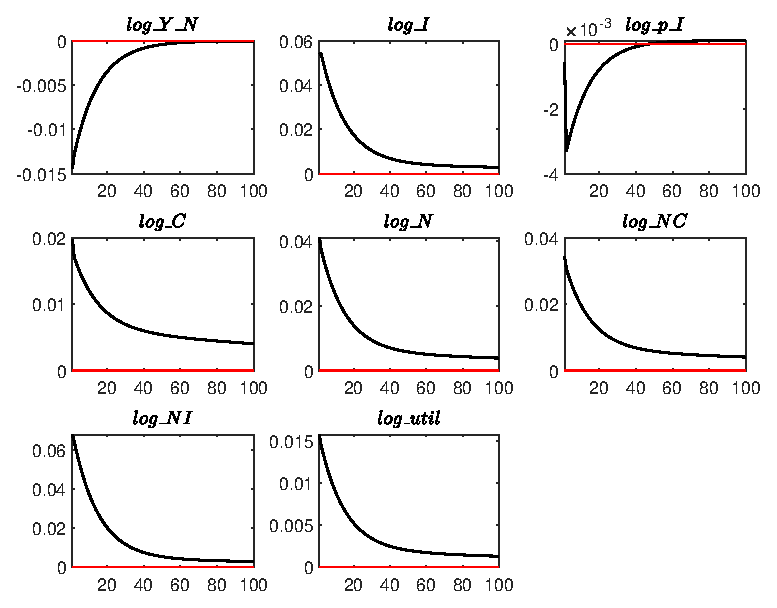
\includegraphics[width=0.80\textwidth]{BRS_imp_mobility_alt/graphs/BRS_imp_mobility_alt_IRF_e_N2}
\caption{Impulse response functions (orthogonalized shock to ${e_N}$).}\label{Fig:IRF:e_N:2}
\end{figure}
 
\begin{figure}[H]
\centering 
\includegraphics[width=0.80\textwidth]{BRS_imp_mobility_alt/graphs/BRS_imp_mobility_alt_IRF_e_D1}
\caption{Impulse response functions (orthogonalized shock to ${e_D}$).}\label{Fig:IRF:e_D:1}
\end{figure}
 
\begin{figure}[H]
\centering 
\includegraphics[width=0.80\textwidth]{BRS_imp_mobility_alt/graphs/BRS_imp_mobility_alt_IRF_e_D2}
\caption{Impulse response functions (orthogonalized shock to ${e_D}$).}\label{Fig:IRF:e_D:2}
\end{figure}
 
\begin{figure}[H]
\centering 
\includegraphics[width=0.80\textwidth]{BRS_imp_mobility_alt/graphs/BRS_imp_mobility_alt_IRF_e_C1}
\caption{Impulse response functions (orthogonalized shock to ${e_C}$).}\label{Fig:IRF:e_C:1}
\end{figure}
 
\begin{figure}[H]
\centering 
\includegraphics[width=0.80\textwidth]{BRS_imp_mobility_alt/graphs/BRS_imp_mobility_alt_IRF_e_C2}
\caption{Impulse response functions (orthogonalized shock to ${e_C}$).}\label{Fig:IRF:e_C:2}
\end{figure}
 
 
% End Of TeX file. 
